\documentclass{ximera}

% These macros are automatically generated from the "macros"
% XML element.  Make permanent edits there.
%
% History
%   2004/01/01  Initiated for FCLA, evolved from there
%   2006/09/17  Converted  _, ^  to \sb, \sp for TeX4ht
%   2014/02/01  Updated for MathBook XML projects
%               Obsolete in FCLA: \codeindent, \computerfont, \define
%               Change: MathJax wants \lt, so replaced by \lteval
%   2014/02/22  New: \orderof, \reals, \per
%   2015/08/16  Incorporated into MathBook XML version of FCLA
%
%%%%%%%%%%%%%%%%%%%%%
%
%     Conveniences
%
%%%%%%%%%%%%%%%%%%%%%
%
%  Order of (asymptotically limit of fraction is 1)
%  Usage: \orderof{some function}
%
\newcommand{\orderof}[1]{\sim #1}
%
%  Integers
%  Usage:  \Z
\newcommand{\Z}{\mathbb{Z}}
%
%  Real numbers, as set of scalars
%  Usage:  \reals
\newcommand{\reals}{\mathbb{R}}
%
%  n-space over real field
%  Usage: \complex{integer-dimension}
\newcommand{\real}[1]{\mathbb{R}^{#1}}
%
%  Complex numbers, as set of scalars
%  Usage:  \complexes
\newcommand{\complexes}{\mathbb{C}}
%
%  n-space over complex field
%  Usage: \complex{integer-dimension}
\newcommand{\complex}[1]{\mathbb{C}^{#1}}
%
%  Complex conjugation (scalar, vector, matrix)
%  Usage: \conjugate{object}
\newcommand{\conjugate}[1]{\overline{#1}}
%
%  Complex number modulus
%  Usage: \modulus{a+bi}
%  Presumes math mode
\newcommand{\modulus}[1]{\left\lvert#1\right\rvert}
%
%  Zero vector
%  Usage: \zerovector
\newcommand{\zerovector}{\vect{0}}
%
%  Zero matrix
%  Usage: \zeromatrix, use a subscript when size is important
\newcommand{\zeromatrix}{\mathcal{O}}
%
%  Inner product (brackets, not quadratic form)
%  Usage: \innerproduct{a-vector}{a-vector}
\newcommand{\innerproduct}[2]{\left\langle#1,\,#2\right\rangle}
%
%  Norm of a vector
%  Usage: \norm{a-vector}
\newcommand{\norm}[1]{\left\lVert#1\right\rVert}
%
%  Dimension
%  Usage: \dimension{vector-space-letter}
\newcommand{\dimension}[1]{\dim\left(#1\right)}
%
%  Nullity
%  Usage: \nullity{matrix-or-lintrans-letter}
\newcommand{\nullity}[1]{n\left(#1\right)}
%
%  Rank
%  Usage: \rank{matrix-or-lintrans-letter}
\newcommand{\rank}[1]{r\left(#1\right)}
%
%  Direct sum
%  Usage: \ds between a couple of subspaces
%
\newcommand{\ds}{\oplus}
%
%  Determinant of a matrix (functional)
%  Usage: \detname{A}
\newcommand{\detname}[1]{\det\left(#1\right)}
%
%  Determinant of a matrix (vertical bars)
%  Usage: \detbars{A}
\newcommand{\detbars}[1]{\left\lvert#1\right\rvert}
%
%  Trace of a Matrix
%  Usage: \trace{matrix name}
\newcommand{\trace}[1]{t\left(#1\right)}
%
%  Square Root of a Matrix
%  Usage: \sr{a-matrix}
\newcommand{\sr}[1]{#1^{1/2}}
%
%%%%%%%%%%%%%%%%%%%%%
%
%     Subspace Constructions
%
%%%%%%%%%%%%%%%%%%%%%
%
%  Span of a set of vectors
%  \span and \sp are used by TeX for other things
%  Usage: \spn{set-of-vectors}
\newcommand{\spn}[1]{\left\langle#1\right\rangle}
%
%  Null space of a matrix
%  Usage:  \nsp{A}
\newcommand{\nsp}[1]{\mathcal{N}\!\left(#1\right)}
%
%  Column space of a matrix
%  Usage:  \csp{A}
\newcommand{\csp}[1]{\mathcal{C}\!\left(#1\right)}
%
%  Row space of a matrix
%  Usage:  \rsp{A}
\newcommand{\rsp}[1]{\mathcal{R}\!\left(#1\right)}
%
%  Left null space of a matrix
%  Usage:  \lns{A}
\newcommand{\lns}[1]{\mathcal{L}\!\left(#1\right)}
%
%  Orthogonal complement of a vector space
%  Avoiding TeX's \perp
%  Usage:  \per{A}
\newcommand{\per}[1]{#1^\perp}
%
%%%%%%%%%%%%%%%%%%%%%
%
%     Systems of Equations
%
%%%%%%%%%%%%%%%%%%%%%
%
%  In-line form of an augmented matrix for a system of equations
%  Usage: \augmented{coefficient-matrix}{constant-vector}
\newcommand{\augmented}[2]{\left\lbrack\left.#1\,\right\rvert\,#2\right\rbrack}
%
%  Notation for a linear system before introducing matrix multiplication
%  Usage: \linearsystem{coefficient-matrix}{constant-vector}
\newcommand{\linearsystem}[2]{\mathcal{LS}\!\left(#1,\,#2\right)}
%
%  Notation for a homogenous system before introducing matrix multiplication
%  Usage: \homosystem{coefficient-matrix}
\newcommand{\homosystem}[1]{\linearsystem{#1}{\zerovector}}
%
%%%%%%%%%%%%%%%%%%%%%
%
%     Row Operations, Echelon Form
%
%%%%%%%%%%%%%%%%%%%%%
%
% Row operations on matrices
%
% Three commands to shorten up descriptions of gaussian elimination
%
% Usage: \rowopswap{row-i}{row-j}
% Usage: \rowopmult{scalar}{row-i}
% Usage: \rowopadd{scalar}{row-multiplied}{row-added-to}
\newcommand{\rowopswap}[2]{R_{#1}\leftrightarrow R_{#2}}
\newcommand{\rowopmult}[2]{#1R_{#2}}
\newcommand{\rowopadd}[3]{#1R_{#2}+R_{#3}}
%
% Mark leading 1's in echelon form with fbox
% Usage: \leading{a-1-usually}
\newcommand{\leading}[1]{\fbox{#1}}
%
%  Row-reduce arrow
%  Usage:  \rref inbetween a matrix and its reduced row-echelon form
\newcommand{\rref}{\xrightarrow{\text{RREF}}}
%
%  Elementary Matrices
%  Usage: \elemswap{subscript}{subscript}
%  Usage: \elemmult{scalar}{subscript}
%  Usage: \elemadd{scalar}{subscript-mult}{subscript-target}
%
\newcommand{\elemswap}[2]{E_{#1,#2}}
\newcommand{\elemmult}[2]{E_{#2}\left(#1\right)}
\newcommand{\elemadd}[3]{E_{#2,#3}\left(#1\right)}
%
%%%%%%%%%%%%%%%%%%%%%
%
%     2-D Constructions (Lists, Vectors, Matrices)
%
%%%%%%%%%%%%%%%%%%%%%
%
%  A list of scalars of generic length
%  Usage:  \scalarlist{scalar letter}{terminal subscript}
\newcommand{\scalarlist}[2]{{#1}_{1},\,{#1}_{2},\,{#1}_{3},\,\ldots,\,{#1}_{#2}}
%
%  Vector styling, bold (or use wiggles, arrows, whatever)
%  Subscripts go outside this construction
%  Usage: \vect{a symbol to use as a vector}
%  Have to already be in math mode
%
\newcommand{\vect}[1]{\mathbf{#1}}
%
%  A column vector
%  Usage: \colvector{list-delimited-by-\\}
%
\newcommand{\colvector}[1]{\begin{bmatrix}#1\end{bmatrix}}
%
%  A generic vector with components
%  Usage: \vectorcomponents{component-letter}{final-subscript}
\newcommand{\vectorcomponents}[2]{\colvector{#1_{1}\\#1_{2}\\#1_{3}\\\vdots\\#1_{#2}}}
%
%  A list of vectors of generic length
%  Usage:  \vectorlist{vector letter}{terminal subscript}
\newcommand{\vectorlist}[2]{\vect{#1}_{1},\,\vect{#1}_{2},\,\vect{#1}_{3},\,\ldots,\,\vect{#1}_{#2}}
%
%  Vector entries, entry i of vector v
%  (vector-expession still needs \vect, etc.)
%  Usage:  \vectorentry{vector-expression}{single-subscript}
\newcommand{\vectorentry}[2]{\left\lbrack#1\right\rbrack_{#2}}
%
%  Matrix entries, entry i,j of matrix A
%  Usage:  \matrixentry{matrix-expression}{paired-subscripts}
%
\newcommand{\matrixentry}[2]{\left\lbrack#1\right\rbrack_{#2}}
%
%  A generic linear combination
%  Usage:  \lincombo{scalar letter}{vector letter}{terminal subscript}
\newcommand{\lincombo}[3]{#1_{1}\vect{#2}_{1}+#1_{2}\vect{#2}_{2}+#1_{3}\vect{#2}_{3}+\cdots +#1_{#3}\vect{#2}_{#3}}
%
%  Matrix, column by column, as vectors
%  Usage:  \matrixcolumns{matrix letter}{terminal subscript}
\newcommand{\matrixcolumns}[2]{\left\lbrack\vect{#1}_{1}|\vect{#1}_{2}|\vect{#1}_{3}|\ldots|\vect{#1}_{#2}\right\rbrack}
%
%%%%%%%%%%%%%%%%%%%%%
%
%     Special Matrices
%
%%%%%%%%%%%%%%%%%%%%%
%
%  Transpose of a matrix
%  Usage:  \transpose{A}
\newcommand{\transpose}[1]{#1^{t}}
%
%  Inverse of a matrix
%  Usage:  \inverse{A}
\newcommand{\inverse}[1]{#1^{-1}}
%
%  Submatrix (for minors, determinants)
%  Usage: \submatrix{matrix-name}{delete-row}{delete-col}
\newcommand{\submatrix}[3]{#1\left(#2|#3\right)}
%
%  Adjoint of a matrix (twice)
%  This macro is a convenience to call \transpose and \conjugate properly
%  It shouldn't need to be modified (or mathematical meanings will change)
%  Usage:  \adj{A}
\newcommand{\adj}[1]{\transpose{\left(\conjugate{#1}\right)}}
%
%  This macro controls the symbol used for the adjoint
%  It can be edited to taste
%  Usage:  \adjoint{A}
\newcommand{\adjoint}[1]{#1^\ast}
%
%%%%%%%%%%%%%%%%%%%%%
%
%     Sets
%
%%%%%%%%%%%%%%%%%%%%%
%
%  A convenience for simple sets
%  Usage:  \set{list of element}
\newcommand{\set}[1]{\left\{#1\right\}}
%
%  Sets with vertical bar, "such that", sized for objects, not condition
%  Usage:  \setparts{objects}{condition}
%
%%\newcommand{\setparts}[2]{\left\{ #1\mid#2\right\}}
%%\newcommand{\setparts}[2]{\left\{\left. #1\right\rvert#2\right\}}
\newcommand{\setparts}[2]{\left\lbrace#1\,\middle|\,#2\right\rbrace}
%
%  Set Cardinality
%  Usage:  \card{a-set-letter}
\newcommand{\card}[1]{\left\lvert#1\right\rvert}
%
%  Set Union
%  Use \cup
%
%  Set Intersection
%  Use \cap
%
%  Set Complement
%  Usage:  \setcomplement{a-set-letter}
\newcommand{\setcomplement}[1]{\overline{#1}}
%
%%%%%%%%%%%%%%%%%%%%%
%
%     Eigenvalues and Eigenspaces
%
%%%%%%%%%%%%%%%%%%%%%
%
%  Characteristic polynomial
%  Usage: \charpoly{matrix-letter}{variable-letter}
\newcommand{\charpoly}[2]{p_{#1}\left(#2\right)}
%
%  Eigenspace
%  Usage: \eigenspace{matrix-letter}{eigenvalue-letter}
\newcommand{\eigenspace}[2]{\mathcal{E}_{#1}\left(#2\right)}
%
%  2013/10/03 Including ampersands is problematic here, 
%  think about fixes later
%  2014/02/22 Limited testing, seems &amp; is fine for HTML and LaTeX
%  2016-07-20 only employed in Archetypes, MBX has gather/align override
%  Eigensystem (presumes wrapped in an mrow within md)
%  Usage: \eigensystem{matrixletter}{eigenvalue}{list of basis vectors}
\newcommand{\eigensystem}[3]{\lambda&amp;=#2&amp;\eigenspace{#1}{#2}&amp;=\spn{\set{#3}}} 
%
%  Generalized Eigenspace
%  Usage: \geneigenspace{lin-trans-letter}{eigenvalue-letter}
\newcommand{\geneigenspace}[2]{\mathcal{G}_{#1}\left(#2\right)}
%
%  Algebraic multiplicty
%  Usage: \algmult{matrix-letter}{eigenvalue-letter}
\newcommand{\algmult}[2]{\alpha_{#1}\left(#2\right)}
%
%  Geometric multiplicty
%  Usage: \geomult{matrix-letter}{eigenvalue-letter}
\newcommand{\geomult}[2]{\gamma_{#1}\left(#2\right)}
%
%  Index (of eigenvalue)
%  Usage: \indx{matrix-letter}{eigenvalue-letter}
\newcommand{\indx}[2]{\iota_{#1}\left(#2\right)}
%
%%%%%%%%%%%%%%%%%%%%%
%
%     Linear Transformations
%
%%%%%%%%%%%%%%%%%%%%%
%
%  MathJax defines \lt to ease XML confusion
%
%  Linear transformation definition
%  Usage: \ltdefn{name-letter}{domain}{range}
\newcommand{\ltdefn}[3]{#1\colon #2\rightarrow#3}
%
%  Linear transformation evaluation
%  Usage: \lteval{name-letter}{input}
%  Replaces old \lt desired by MathJax
\newcommand{\lteval}[2]{#1\left(#2\right)}
%
% Linear transformation inverse
%  Usage: \ltinverse{name-letter}
\newcommand{\ltinverse}[1]{#1^{-1}}
%
%  Linear transformation restriction
%  Usage: \restrict{name-letter}{subspace-letter}
\newcommand{\restrict}[2]{{#1}|_{#2}}
%
%  Linear transformation preimage
%  Usage: \preimage{name-letter}{codomain-element}
\newcommand{\preimage}[2]{#1^{-1}\left(#2\right)}
%
%  Range of a linear transformation
%  TeX uses \range for something else
%  Usage:  \rng{T}
\newcommand{\rng}[1]{\mathcal{R}\!\left(#1\right)}
%
%  Kernel of a linear transformation
%  TeX uses \ker to do something different
%  Usage:  \krn{T}
\newcommand{\krn}[1]{\mathcal{K}\!\left(#1\right)}
%
%  Linear transformation composition
%  Usage: \compose{function-name}{function-name}
\newcommand{\compose}[2]{{#1}\circ{#2}}
%
%  Vector space of linear transformations
%  Usage: \vslt{domains}{codomains}
%  Presumes math mode
\newcommand{\vslt}[2]{\mathcal{LT}\left(#1,\,#2\right)}
%
%%%%%%%%%%%%%%%%%%%%%
%
%     Vector and Matrix Representations
%
%%%%%%%%%%%%%%%%%%%%%
%
%  Isomorphism symbol
%  Usage: \isomorphic
\newcommand{\isomorphic}{\cong}
%
%  Similarity
%  Usage: \similar{inner-matrix}{outer-invertible-matrix}
%  Rearranging this will not "fix" all desired changes throughout
%
\newcommand{\similar}[2]{\inverse{#2}#1#2}
%
%  Vector representation function name
%  Usage: \vectrepname{basis-letter}
\newcommand{\vectrepname}[1]{\rho_{#1}}
%
%  Vector representation output
%  Usage: \vectrep{basis-letter}{input}
\newcommand{\vectrep}[2]{\lteval{\vectrepname{#1}}{#2}}
%
%  Vector representation inverse function name
%  (Added later, not used consistently in FCLA)
%  Usage: \vectrepinvname{basis-letter}
\newcommand{\vectrepinvname}[1]{\ltinverse{\vectrepname{#1}}}
%
%  Vector representation inverse output
%  Usage: \vectrepinv{basis-letter}{input}
\newcommand{\vectrepinv}[2]{\lteval{\ltinverse{\vectrepname{#1}}}{#2}}
%
%  Matrix representation
%  Usage: \matrixrep{transformation-letter}{domain-basis-letter}{codomain-basis-letter}
\newcommand{\matrixrep}[3]{M^{#1}_{#2,#3}}
%
%  Matrix representation column-by-colum
%  2016-07-20 only employed once?
%  Usage: \matrixrepcolumns{transformation-letter}{codomain-basis-letter}{codomain-basis-vector-letter}{final-index}
\newcommand{\matrixrepcolumns}[4]{\left\lbrack \left.\vectrep{#2}{\lteval{#1}{\vect{#3}_{1}}}\right|\left.\vectrep{#2}{\lteval{#1}{\vect{#3}_{2}}}\right|\left.\vectrep{#2}{\lteval{#1}{\vect{#3}_{3}}}\right|\ldots\left|\vectrep{#2}{\lteval{#1}{\vect{#3}_{#4}}}\right.\right\rbrack}
%
%  Change of basis matrix
%  Usage: \cbm{domain-basis-letter}{codomain-basis-letter}
\newcommand{\cbm}[2]{C_{#1,#2}}
%
%%%%%%%%%%%%%%%%%%%%%
%
%     Canonical Forms
%
%%%%%%%%%%%%%%%%%%%%%
%
%  Jordan blocks
%  Usage: \jordan{size}{diagonal-element}
\newcommand{\jordan}[2]{J_{#1}\left(#2\right)}
%
%%%%%%%%%%%%%%%%%%%%%
%
%     Hadamard Matrices
%     Contributed by Elizabeth Million
%
%%%%%%%%%%%%%%%%%%%%%
%
%  Hadamard Product
%  Usage: \hadamard{a-matrix}{a-matrix}
\newcommand{\hadamard}[2]{#1\circ #2}
%
%  Hadamard identity matrix
%  Usage: \hadamardidentity{paired-subscripts-size-of-matrix}
\newcommand{\hadamardidentity}[1]{J_{#1}}
%
%  Hadamard inverse matrix
%  Usage: \hadamardinverse{matrix-expression}
\newcommand{\hadamardinverse}[1]{\widehat{#1}}


\title{Four Subsets}

\begin{document}
\begin{abstract}
  We can find linearly independent sets to describe the null space,
  column space, row space, left null space by analyzing only the
  extended echelon form of the matrix.
\end{abstract}
\maketitle

With all the preliminaries in place we can state a theorem. In
essence, this result will allow us to say that we can find linearly
independent sets to use in span constructions for all four subsets
(null space, column space, row space, left null space) by analyzing
only the extended echelon form of the matrix, and specifically, just
the two submatrices $C$ and $L$, which will be ripe for analysis since
they are already in reduced row-echelon form (\ref{theorem:PEEF}).

\begin{theorem}[Four Subsets]
\label{theorem:FS}
Suppose $A$ is an $m\times n$ matrix with extended echelon form $N$.
Suppose the reduced row-echelon form of $A$ has $r$ nonzero rows.
Then $C$ is the submatrix of $N$ formed from the first $r$ rows and
the first $n$ columns and $L$ is the submatrix of $N$ formed from the
last $m$ columns and the last $m-r$ rows.  Then
\begin{enumerate}
\item The null space of $A$ is the null space of $C$, $\nsp{A}=\nsp{C}$.
\item The row space of $A$ is the row space of $C$, $\rsp{A}=\rsp{C}$.
\item The column space of $A$ is the null space of $L$, $\csp{A}=\nsp{L}$.
\item The left null space of $A$ is the row space of $L$, $\lns{A}=\rsp{L}$.
\end{enumerate}

\begin{proof}
  First, $\nsp{A}=\nsp{B}$ since $B$ is row-equivalent to $A$
  (\ref{theorem:REMES}).  The zero rows of $B$ represent equations
  that are always true in the homogeneous system $\homosystem{B}$, so
  the removal of these equations will not change the solution set.
  Thus, in turn, $\nsp{B}=\nsp{C}$.

  Second, $\rsp{A}=\rsp{B}$ since $B$ is row-equivalent to $A$
  (\ref{theorem:REMRS}).  The zero rows of $B$ contribute nothing to
  the span that is the row space of $B$, so the removal of these rows
  will not change the row space.  Thus, in turn, $\rsp{B}=\rsp{C}$.

  Third, we prove the set equality $\csp{A}=\nsp{L}$ with
  \ref{definition:SE}.  Begin by showing that
  $\csp{A}\subseteq\nsp{L}$.  Choose
  $\vect{y}\in\csp{A}\subseteq\complex{m}$.  Then there exists a
  vector $\vect{x}\in\complex{n}$ such that $A\vect{x}=\vect{y}$
  (\ref{theorem:CSCS}).  Then for $1\leq k\leq m-r$,
  \begin{align*}
    \vectorentry{L\vect{y}}{k}
    &=\vectorentry{J\vect{y}}{r+k}
    &&\text{$L$ a submatrix of $J$}\\
    &=\vectorentry{B\vect{x}}{r+k}
    &&\ref{theorem:PEEF}\\
    &=\vectorentry{\zeromatrix\vect{x}}{k}
    &&\text{Zero matrix a submatrix of $B$}\\
    &=\vectorentry{\zerovector}{k}
    &&\ref{theorem:MMZM}
  \end{align*}
  
  So, for all $1\leq k\leq m-r$,
  $\vectorentry{L\vect{y}}{k}=\vectorentry{\zerovector}{k}$.  So by
  \ref{definition:CVE} we have $L\vect{y}=\zerovector$ and thus
  $\vect{y}\in\nsp{L}$.

  Now, show that $\nsp{L}\subseteq\csp{A}$.  Choose
  $\vect{y}\in\nsp{L}\subseteq\complex{m}$.  Form the vector
  $K\vect{y}\in\complex{r}$.  The linear system
  $\linearsystem{C}{K\vect{y}}$ is consistent since $C$ is in reduced
  row-echelon form and has no zero rows (\ref{theorem:PEEF}).  Let
  $\vect{x}\in\complex{n}$ denote a solution to
  $\linearsystem{C}{K\vect{y}}$.

  Then for $1\leq j\leq r$,
  \begin{align*}
    \vectorentry{B\vect{x}}{j}
    &=\vectorentry{C\vect{x}}{j}
    &&\text{$C$ a submatrix of $B$}\\
    &=\vectorentry{K\vect{y}}{j}
    &&\text{$\vect{x}$ a solution to $\linearsystem{C}{K\vect{y}}$}\\
    &=\vectorentry{J\vect{y}}{j}
    &&\text{$K$ a submatrix of $J$}\\
  \end{align*}
  
  And for $r+1\leq k\leq m$,
  \begin{align*}
    \vectorentry{B\vect{x}}{k}
    &=\vectorentry{\zeromatrix\vect{x}}{k-r}
    &&\text{Zero matrix a submatrix of $B$}\\
    &=\vectorentry{\zerovector}{k-r}
    &&\ref{theorem:MMZM}\\
    &=\vectorentry{L\vect{y}}{k-r}
    &&\text{$\vect{y}$ in $\nsp{L}$}\\
    &=\vectorentry{J\vect{y}}{k}
    &&\text{$L$ a submatrix of $J$}\\
  \end{align*}
  
  So for all $1\leq i\leq m$,
  $\vectorentry{B\vect{x}}{i}=\vectorentry{J\vect{y}}{i}$ and by
  \ref{definition:CVE} we have $B\vect{x}=J\vect{y}$.  From
  \ref{theorem:PEEF} we know then that $A\vect{x}=\vect{y}$, and
  therefore $\vect{y}\in\csp{A}$ (\ref{theorem:CSCS}).  By
  \ref{definition:SE} we now have $\csp{A}=\nsp{L}$.

  Fourth, we prove the set equality $\lns{A}=\rsp{L}$ with
  \ref{definition:SE}.  Begin by showing that
  $\rsp{L}\subseteq\lns{A}$.  Choose
  $\vect{y}\in\rsp{L}\subseteq\complex{m}$.  Then there exists a
  vector $\vect{w}\in\complex{m-r}$ such that
  $\vect{y}=\transpose{L}\vect{w}$ (\ref{definition:RSM},
  \ref{theorem:CSCS}).  Then for $1\leq i\leq n$,
  \begin{align*}
    \vectorentry{\transpose{A}\vect{y}}{i}
    &=\sum_{k=1}^{m}\matrixentry{\transpose{A}}{ik}\vectorentry{\vect{y}}{k}
    &&\ref{theorem:EMP}\\
    &=\sum_{k=1}^{m}\matrixentry{\transpose{A}}{ik}\vectorentry{\transpose{L}\vect{w}}{k}
    &&\text{Definition of $\vect{w}$}\\
    &=\sum_{k=1}^{m}\matrixentry{\transpose{A}}{ik}\sum_{\ell=1}^{m-r}\matrixentry{\transpose{L}}{k\ell}\vectorentry{\vect{w}}{\ell}
    &&\ref{theorem:EMP}\\
    &=\sum_{k=1}^{m}\sum_{\ell=1}^{m-r}\matrixentry{\transpose{A}}{ik}\matrixentry{\transpose{L}}{k\ell}\vectorentry{\vect{w}}{\ell}
    &&\ref{property:DCN}\\
    &=\sum_{\ell=1}^{m-r}\sum_{k=1}^{m}\matrixentry{\transpose{A}}{ik}\matrixentry{\transpose{L}}{k\ell}\vectorentry{\vect{w}}{\ell}
    &&\ref{property:CACN}\\
    &=\sum_{\ell=1}^{m-r}\left(\sum_{k=1}^{m}\matrixentry{\transpose{A}}{ik}\matrixentry{\transpose{L}}{k\ell}\right)\vectorentry{\vect{w}}{\ell}
    &&\ref{property:DCN}\\
    &=\sum_{\ell=1}^{m-r}\left(\sum_{k=1}^{m}\matrixentry{\transpose{A}}{ik}\matrixentry{\transpose{J}}{k,r+\ell}\right)\vectorentry{\vect{w}}{\ell}
    &&\text{$L$ a submatrix of $J$}\\
    &=\sum_{\ell=1}^{m-r}\matrixentry{\transpose{A}\transpose{J}}{i,r+\ell}\vectorentry{\vect{w}}{\ell}
    &&\ref{theorem:EMP}\\
    &=\sum_{\ell=1}^{m-r}\matrixentry{\transpose{\left(JA\right)}}{i,r+\ell}\vectorentry{\vect{w}}{\ell}
    &&\ref{theorem:MMT}\\
    &=\sum_{\ell=1}^{m-r}\matrixentry{\transpose{B}}{i,r+\ell}\vectorentry{\vect{w}}{\ell}
    &&\ref{theorem:PEEF}\\
    &=\sum_{\ell=1}^{m-r}0\vectorentry{\vect{w}}{\ell}
    &&\text{Zero rows in $B$}\\
    &=0
    &&\ref{property:ZCN}\\
    &=\vectorentry{\zerovector}{i}
    &&\ref{definition:ZCV}
  \end{align*}
  
  Since
  $\vectorentry{\transpose{A}\vect{y}}{i}=\vectorentry{\zerovector}{i}$
  for $1\leq i\leq n$, \ref{definition:CVE} implies that
  $\transpose{A}\vect{y}=\zerovector$.  This means that
  $\vect{y}\in\nsp{\transpose{A}}$.

  Now, show that $\lns{A}\subseteq\rsp{L}$.  Choose
  $\vect{y}\in\lns{A}\subseteq\complex{m}$.  The matrix $J$ is
  nonsingular (\ref{theorem:PEEF}), so $\transpose{J}$ is also
  nonsingular (\ref{theorem:MIT}) and therefore the linear system
  $\linearsystem{\transpose{J}}{\vect{y}}$ has a unique solution.
  Denote this solution as $\vect{x}\in\complex{m}$.  We will need to
  work with two ``halves'' of $\vect{x}$, which we will denote as
  $\vect{z}$ and $\vect{w}$ with formal definitions given by
  \begin{align*}
    \vectorentry{z}{j}&=\vectorentry{x}{i}
    &
    &1\leq j\leq r,
    &&&
        \vectorentry{w}{k}&=\vectorentry{x}{r+k}
    &
    &1\leq k\leq m-r
  \end{align*}

  Now, for $1\leq j\leq r$,
  \begin{align*}
    \vectorentry{\transpose{C}\vect{z}}{j}
    &=\sum_{k=1}^{r}\matrixentry{\transpose{C}}{jk}\vectorentry{\vect{z}}{k}
    &&\ref{theorem:EMP}\\
    &=\sum_{k=1}^{r}\matrixentry{\transpose{C}}{jk}\vectorentry{\vect{z}}{k}+
      \sum_{\ell=1}^{m-r}\matrixentry{\zeromatrix}{j\ell}\vectorentry{\vect{w}}{\ell}
    &&\ref{definition:ZM}\\
    &=\sum_{k=1}^{r}\matrixentry{\transpose{B}}{jk}\vectorentry{\vect{z}}{k}+
      \sum_{\ell=1}^{m-r}\matrixentry{\transpose{B}}{j,r+\ell}\vectorentry{\vect{w}}{\ell}
    &&\text{$C$, $\zeromatrix$ submatrices of $B$}\\
    &=\sum_{k=1}^{r}\matrixentry{\transpose{B}}{jk}\vectorentry{\vect{x}}{k}+
      \sum_{\ell=1}^{m-r}\matrixentry{\transpose{B}}{j,r+\ell}\vectorentry{\vect{x}}{r+\ell}
    &&\text{Definitions of $\vect{z}$ and $\vect{w}$}\\
    &=\sum_{k=1}^{r}\matrixentry{\transpose{B}}{jk}\vectorentry{\vect{x}}{k}+
      \sum_{k=r+1}^{m}\matrixentry{\transpose{B}}{jk}\vectorentry{\vect{x}}{k}
    &&\text{Re-index second sum}\\
    &=\sum_{k=1}^{m}\matrixentry{\transpose{B}}{jk}\vectorentry{\vect{x}}{k}
    &&\text{Combine sums}\\
    &=\sum_{k=1}^{m}\matrixentry{\transpose{\left(JA\right)}}{jk}\vectorentry{\vect{x}}{k}
    &&\ref{theorem:PEEF}\\
    &=\sum_{k=1}^{m}\matrixentry{\transpose{A}\transpose{J}}{jk}\vectorentry{\vect{x}}{k}
    &&\ref{theorem:MMT}\\
    &=\sum_{k=1}^{m}\sum_{\ell=1}^{m}\matrixentry{\transpose{A}}{j\ell}\matrixentry{\transpose{J}}{\ell k}\vectorentry{\vect{x}}{k}
    &&\ref{theorem:EMP}\\
    &=\sum_{\ell=1}^{m}\sum_{k=1}^{m}\matrixentry{\transpose{A}}{j\ell}\matrixentry{\transpose{J}}{\ell k}\vectorentry{\vect{x}}{k}
    &&\ref{property:CACN}\\
    &=\sum_{\ell=1}^{m}\matrixentry{\transpose{A}}{j\ell}\left(\sum_{k=1}^{m}\matrixentry{\transpose{J}}{\ell k}\vectorentry{\vect{x}}{k}\right)
    &&\ref{property:DCN}\\
    &=\sum_{\ell=1}^{m}\matrixentry{\transpose{A}}{j\ell}\vectorentry{\transpose{J}\vect{x}}{\ell}
    &&\ref{theorem:EMP}\\
    &=\sum_{\ell=1}^{m}\matrixentry{\transpose{A}}{j\ell}\vectorentry{\vect{y}}{\ell}
    &&\text{Definition of $\vect{x}$}\\
    &=\vectorentry{\transpose{A}\vect{y}}{j}
    &&\ref{theorem:EMP}\\
    &=\vectorentry{\zerovector}{j}
    &&\text{$\vect{y}\in\lns{A}$}
  \end{align*}
  
  So, by \ref{definition:CVE}, $\transpose{C}\vect{z}=\zerovector$ and
  the vector $\vect{z}$ gives us a linear combination of the columns
  of $\transpose{C}$ that equals the zero vector.  In other words,
  $\vect{z}$ gives a relation of linear dependence on the the rows of
  $C$.  However, the rows of $C$ are a linearly independent set by
  \ref{theorem:BRS}.  According to \ref{definition:LICV} we must
  conclude that the entries of $\vect{z}$ are all zero, i.e.,
  $\vect{z}=\zerovector$.

  Now, for $1\leq i\leq m$, we have
  \begin{align*}
    \vectorentry{\vect{y}}{i}
    &=\vectorentry{\transpose{J}\vect{x}}{i}
    &&\text{Definition of $\vect{x}$}\\
    &=\sum_{k=1}^{m}\matrixentry{\transpose{J}}{ik}\vectorentry{\vect{x}}{k}
    &&\ref{theorem:EMP}\\
    &=\sum_{k=1}^{r}\matrixentry{\transpose{J}}{ik}\vectorentry{\vect{x}}{k}+
      \sum_{k=r+1}^{m}\matrixentry{\transpose{J}}{ik}\vectorentry{\vect{x}}{k}
    &&\text{Break apart sum}\\
    &=\sum_{k=1}^{r}\matrixentry{\transpose{J}}{ik}\vectorentry{\vect{z}}{k}+
      \sum_{k=r+1}^{m}\matrixentry{\transpose{J}}{ik}\vectorentry{\vect{w}}{k-r}
    &&\text{Definition of $\vect{z}$ and $\vect{w}$}\\
    &=\sum_{k=1}^{r}\matrixentry{\transpose{J}}{ik}0+
      \sum_{\ell=1}^{m-r}\matrixentry{\transpose{J}}{i,r+\ell}\vectorentry{\vect{w}}{\ell}
    &&\text{$\vect{z}=\zerovector$, re-index}\\
    &=0+\sum_{\ell=1}^{m-r}\matrixentry{\transpose{L}}{i,\ell}\vectorentry{\vect{w}}{\ell}
    &&\text{$L$ a submatrix of $J$}\\
    &=\vectorentry{\transpose{L}\vect{w}}{i}
    &&\ref{theorem:EMP}\\
  \end{align*}

  So by \ref{definition:CVE}, $\vect{y}=\transpose{L}\vect{w}$.  The
  existence of $\vect{w}$ implies that $\vect{y}\in\rsp{L}$, and
  therefore $\lns{A}\subseteq\rsp{L}$.  So by \ref{definition:SE} we
  have $\lns{A}=\rsp{L}$.

\end{proof}
\end{theorem}

The first two conclusions of this theorem are nearly trivial.  But
they set up a pattern of results for $C$ that is reflected in the
latter two conclusions about $L$.  In total, they tell us that we can
compute all four subsets just by finding null spaces and row spaces.
This theorem does not tell us exactly how to compute these subsets,
but instead simply expresses them as null spaces and row spaces of
matrices in reduced row-echelon form without any zero rows ($C$ and
$L$).  A linearly independent set that spans the null space of a
matrix in reduced row-echelon form can be found easily with
\ref{theorem:BNS}.  It is an even easier matter to find a linearly
independent set that spans the row space of a matrix in reduced
row-echelon form with \ref{theorem:BRS}, especially when there are no
zero rows present.  So an application of \ref{theorem:FS} is typically
followed by two applications each of \ref{theorem:BNS} and
\ref{theorem:BRS}.

The situation when $r=m$ deserves comment, since now the matrix $L$
has no rows.  What is $\csp{A}$ when we try to apply \ref{theorem:FS}
and encounter $\nsp{L}$?  One interpretation of this situation is that
$L$ is the coefficient matrix of a homogeneous system that has no
equations.  How hard is it to find a solution vector to this system?
Some thought will convince you that \textit{any} proposed vector will
qualify as a solution, since it makes \textit{all} of the equations
true.  So every possible vector is in the null space of $L$ and
therefore $\csp{A}=\nsp{L}=\complex{m}$.  Perhaps you are not
convinced?  Let us try another argument that might solidly convince
you of this logic.

If $r=m$, when we row-reduce the augmented matrix of
$\linearsystem{A}{\vect{b}}$ the result will have no zero rows, and
the first $n$ columns will all be pivot columns, leaving none for the
final column, so by \ref{theorem:RCLS} the system will be consistent.
By \ref{theorem:CSCS}, $\vect{b}\in\csp{A}$.  Since $\vect{b}$ was
arbitrary, every possible vector is in the column space of $A$, so we
again have $\csp{A}=\complex{m}$.  The situation when a matrix has
$r=m$ is known by the term \dfn{full rank}, and in the case of a
square matrix coincides with nonsingularity.

The properties of the matrix $L$ described by this theorem can be
explained informally as follows.  A column vector
$\vect{y}\in\complex{m}$ is in the column space of $A$ if the linear
system $\linearsystem{A}{\vect{y}}$ is consistent
(\ref{theorem:CSCS}).  By \ref{theorem:RCLS}, the reduced row-echelon
form of the augmented matrix $\augmented{A}{\vect{y}}$ of a consistent
system will have zeros in the bottom $m-r$ locations of the last
column.  By \ref{theorem:PEEF} this final column is the vector
$J\vect{y}$ and so should then have zeros in the final $m-r$
locations.  But since $L$ comprises the final $m-r$ rows of $J$, this
condition is expressed by saying $\vect{y}\in\nsp{L}$.

Additionally, the rows of $J$ are the scalars in linear combinations
of the rows of $A$ that create the rows of $B$.  That is, the rows of
$J$ record the net effect of the sequence of row operations that takes
$A$ to its reduced row-echelon form, $B$.  This can be seen in the
equation $JA=B$ (\ref{theorem:PEEF}).  As such, the rows of $L$ are
scalars for linear combinations of the rows of $A$ that yield zero
rows.  But such linear combinations are precisely the elements of the
left null space.  So any element of the row space of $L$ is also an
element of the left null space of $A$.

We will now illustrate \ref{theorem:FS} with a few examples.

\begin{example}[Four subsets, no. 1]

  In \ref{example:SEEF} we found the five relevant submatrices of the
  extended echelon form for the matrix
  \[
    A=
    \begin{bmatrix}
      1 & -1 & -2 & 7 & 1 & 6 \\
      -6 & 2 & -4 & -18 & -3 & -26 \\
      4 & -1 & 4 & 10 & 2 & 17 \\
      3 & -1 & 2 & 9 & 1 & 12
    \end{bmatrix}
  \]
  
  To apply \ref{theorem:FS} we only need $C$ and $L$,
  \begin{align*}
    C&=
       \begin{bmatrix}
         \leading{1} &                0 & 2 & 1 &                0 & 3 \\
         0 & \leading{1} & 4 & -6 &               0 & -1 \\
         0 &                0 & 0 & 0 & \leading{1} & 2
       \end{bmatrix}
                                                                   &
                                                                     L&=
                                                                        \begin{bmatrix}
                                                                          \leading{1} & 2 & 2 & 1
                                                                        \end{bmatrix}
  \end{align*}
  
  Then we use \ref{theorem:FS}  to obtain
  \begin{align*}
    \nsp{A}&=\nsp{C}=
             \spn{\set{
             \colvector{-2\\-4\\1\\0\\0\\0},\,
    \colvector{-1\\6\\0\\1\\0\\0},\,
    \colvector{-3\\1\\0\\0\\-2\\1}
    }}
           &&\ref{theorem:BNS}\\
    \rsp{A}&=\rsp{C}=
             \spn{\set{
             \colvector{1\\0\\2\\1\\0\\3 },\,
    \colvector{0\\1\\4\\-6\\0\\-1},\,
    \colvector{0\\0\\0\\0\\1\\2}
    }}
           &&\ref{theorem:BRS}\\
    \csp{A}&=\nsp{L}=
             \spn{\set{
             \colvector{-2\\1\\0\\0},\,
    \colvector{-2\\0\\1\\0},\,
    \colvector{-1\\0\\0\\1}
    }}
           &&\ref{theorem:BNS}\\
    \lns{A}&=\rsp{L}=
             \spn{\set{
             \colvector{1\\2\\2\\1}
    }}
           &&\ref{theorem:BRS}
  \end{align*}

  Boom!
\end{example}

\begin{example}[Four subsets, no. 2]

  Now let us return to the matrix $A$ that we used to motivate this section in \ref{example:CSANS},
  \[
    A=
    \begin{bmatrix}
      10 & 0 & 3 & 8 & 7 \\
      -16 & -1 & -4 & -10 & -13 \\
      -6 & 1 & -3 & -6 & -6 \\
      0 & 2 & -2 & -3 & -2 \\
      3 & 0 & 1 & 2 & 3 \\
      -1 & -1 & 1 & 1 & 0
    \end{bmatrix}
  \]

  We form the matrix $M$ by adjoining the $6\times 6$ identity matrix $I_6$,
  \[
    M=
    \left[\begin{array}{@{}*{12}{c}@{}}
      10 & 0 & 3 & 8 & 7 & 1 & 0 & 0 & 0 & 0 & 0 \\
      -16 & -1 & -4 & -10 & -13 & 0 & 1 & 0 & 0 & 0 & 0 \\
      -6 & 1 & -3 & -6 & -6 & 0 & 0 & 1 & 0 & 0 & 0 \\
      0 & 2 & -2 & -3 & -2 & 0 & 0 & 0 & 1 & 0 & 0 \\
      3 & 0 & 1 & 2 & 3 & 0 & 0 & 0 & 0 & 1 & 0 \\
      -1 & -1 & 1 & 1 & 0 & 0 & 0 & 0 & 0 & 0 & 1
    \end{array}\right]
  \]
  and row-reduce to obtain $N$
  \[
    N=
    \left[\begin{array}{@{}*{12}{c}@{}}
      \leading{1} & 0 & 0 & 0 & 2 & 0 & 0 & 1 & -1 & 2 & -1 \\
      0 & \leading{1} & 0 & 0 & -3 & 0 & 0 & -2 & 3 & -3 & 3 \\
      0 & 0 & \leading{1} & 0 & 1 & 0 & 0 & 1 & 1 & 3 & 3 \\
      0 & 0 & 0 & \leading{1} & -2 & 0 & 0 & -2 & 1 & -4 & 0 \\
      0 & 0 & 0 & 0 & 0 & \leading{1} & 0 & 3 & -1 & 3 & 1 \\
      0 & 0 & 0 & 0 & 0 & 0 & \leading{1} & -2 & 1 & 1 & -1
          \end{array}\right]
  \]
  
  To find the four subsets for $A$, we only need identify the
  $4\times 5$ matrix $C$ and the $2\times 6$ matrix $L$,
  \begin{align*}
    C&=
       \begin{bmatrix}
         \leading{1} & 0 & 0 & 0 & 2\\
         0 & \leading{1} & 0 & 0 & -3\\
         0 & 0 & \leading{1} & 0 & 1\\
         0 & 0 & 0 & \leading{1} & -2
       \end{bmatrix}
                                 &
                                   L&=
                                      \begin{bmatrix}
                                        \leading{1} & 0 & 3 & -1 & 3 & 1 \\
                                        0 & \leading{1} & -2 & 1 & 1 & -1
                                      \end{bmatrix}
  \end{align*}

  Then we apply \ref{theorem:FS},
  \begin{align*}
    \nsp{A}&=\nsp{C}=
             \spn{\set{
             \colvector{-2\\3\\-1\\2\\1}
    }}
           &&\ref{theorem:BNS}\\
    \rsp{A}&=\rsp{C}=
             \spn{\set{
             \colvector{1 \\ 0 \\ 0 \\ 0 \\ 2},\,
    \colvector{0 \\ 1 \\ 0 \\ 0 \\ -3},\,
    \colvector{0 \\ 0 \\ 1 \\ 0 \\ 1},\,
    \colvector{0 \\ 0 \\ 0 \\ 1 \\ -2}
    }}
           &&\ref{theorem:BRS}\\
    \csp{A}&=\nsp{L}=
             \spn{\set{
             \colvector{-3\\2\\1\\0\\0\\0},\,
    \colvector{1\\-1\\0\\1\\0\\0},\,
    \colvector{-3\\-1\\0\\0\\1\\0},\,
    \colvector{-1\\1\\0\\0\\0\\1}
    }}
           &&\ref{theorem:BNS}\\
    \lns{A}&=\rsp{L}=
             \spn{\set{
             \colvector{1 \\ 0 \\ 3 \\ -1 \\ 3 \\ 1},\,
    \colvector{0 \\ 1 \\ -2 \\ 1 \\ 1 \\ -1}
    }}
           &&\ref{theorem:BRS}
  \end{align*}
\end{example}

The next example is just a bit different since the matrix has more
rows than columns, and a trivial null space.

\begin{example}[Four subsets]
  Consider a system of $m=5$ equations in $n=2$ variables with coefficient matrix
  \[
    G=
    \begin{bmatrix}
      2 & 3\\
      -1 & 4 \\
      3 & 10\\
      3 &  -1\\
      6 & 9
    \end{bmatrix}
  \]

  Adjoin the $5\times 5$ identity matrix, $I_5$, to form
  \[
    M=
    \begin{bmatrix}
      2 & 3 & 1&0&0&0&0\\
      -1 & 4 & 0&1&0&0&0\\
      3 & 10 & 0&0&1&0&0\\
      3 &  -1 & 0&0&0&1&\answer{0}\\
      6 & 9 & 0&0&0&0&\answer{1}
    \end{bmatrix}
  \]

  This row-reduces to
  \[
    N=
    \begin{bmatrix}
      \leading{1} & 0 & 0 & 0 & 0 & \frac{3}{11} & \frac{1}{33}\\
      0 & \leading{1} & 0 & 0 & 0 & -\frac{2}{11} & \frac{1}{11}\\
      0 & 0 & \leading{1} & 0 & 0 & 0 & -\frac{1}{3}\\
      0 & 0 & 0 & \leading{1} & 0 & 1 & -\frac{1}{3}\\
      0 & 0 & 0 & 0 & \leading{1} & 1 & -1
    \end{bmatrix}
  \]

  The first $n=2$ columns contain $r=\answer{2}$ leading 1's, so we
  obtain $C$ as the $2\times 2$ identity matrix and extract $L$ from
  the final $m-r=3$ rows in the final $m=5$ columns.
  \begin{align*}
    C&=
       \begin{bmatrix}
         \leading{1} & 0\\
         0 & \leading{1}
       \end{bmatrix}
                     &
                       L&=
                          \begin{bmatrix}
                            \leading{1} & 0 & 0 & 0 & -\frac{1}{3}\\
                            0 & \leading{1}  & 0 & 1 & -\frac{1}{3}\\
                            0 & 0 & \leading{1}  & 1 & -1
                          \end{bmatrix}
  \end{align*}
  
  Then we apply \ref{theorem:FS},
  \begin{align*}
    \nsp{G}=\nsp{C}&=
                     \spn{\emptyset}
                     =\set{\zerovector}
    &&\ref{theorem:BNS}\\
    \rsp{G}=\rsp{C}&=
                     \spn{\set{
                     \colvector{1 \\ 0},\,
    \colvector{0 \\ 1}
    }}
    =\complex{2}
                   &&\ref{theorem:BRS}\\
    \csp{G}=\nsp{L}&=
                     \spn{\set{
                     \colvector{0\\-1\\-1\\1\\0},\,
    \colvector{\frac{1}{3}\\\frac{1}{3}\\1\\0\\1}
    }}&&\ref{theorem:BNS}\\
                   &=\spn{\set{
                     \colvector{0\\-1\\-1\\1\\0},\,
    \colvector{1\\1\\3\\0\\3}
    }}\\
    \lns{G}=\rsp{L}&=
                     \spn{\set{
                     \colvector{1 \\ 0 \\ 0 \\ 0 \\ -\frac{1}{3}},\,
    \colvector{0 \\ 1  \\ 0 \\ 1 \\ -\frac{1}{3}},\,
    \colvector{0 \\ 0 \\ 1  \\ 1 \\ -1}
    }}&&\ref{theorem:BRS}\\
                   &=\spn{\set{
                     \colvector{3 \\ 0 \\ 0 \\ 0 \\ -1},\,
    \colvector{0 \\ 3  \\ 0 \\ 3\ \\ -1},\,
    \colvector{0 \\ 0 \\ 1  \\ 1 \\ -1}
    }}
  \end{align*}

  Depending on the choice of $\vec{b}$, the linear system
  $\linearsystem{G}{\vec{b}}$ may or may not be consistent.  See if
  you can write the two different vectors of constants from these two
  archetypes as linear combinations of the two vectors that form the
  spanning set for $\csp{G}$.  How about the two columns of $G$?  Can
  you write each individually as a linear combination of the two
  vectors that form the spanning set for $\csp{G}$?  They must be in
  the column space of $G$ also.  Are your answers unique?  Do you
  notice anything about the scalars that appear in the linear
  combinations you are forming?
\end{example}

So we have three different methods to obtain a description of the
column space of a matrix as the span of a linearly independent set.
\ref{theorem:BCS} is sometimes useful since the vectors it specifies
are equal to actual columns of the matrix. \ref{theorem:BRS} and
\ref{theorem:CSRST} combine to create vectors with lots of zeros, and
strategically placed 1's near the top of the vector.  \ref{theorem:FS}
and the matrix $L$ from the extended echelon form gives us a third
method, which tends to create vectors with lots of zeros, and
strategically placed 1's near the bottom of the vector.  If we do not
care about linear independence we can also appeal to
\ref{definition:CSM} and simply express the column space as the span
of all the columns of the matrix, giving us a fourth description.


With \ref{theorem:CSRST} and \ref{definition:RSM}, we can compute
column spaces with theorems about row spaces, and we can compute row
spaces with theorems about column spaces, but in each case we must
transpose the matrix first.  At this point you may be overwhelmed by
all the possibilities for computing column and row spaces.
\ref{diagram:CSRST} is meant to help.  For both the column space and
row space, it suggests four techniques.  One is to appeal to the
definition, another yields a span of a linearly independent set, and a
third uses \ref{theorem:FS}.  A fourth suggests transposing the matrix
and the dashed line implies that then the companion set of techniques
can be applied.  This can lead to a bit of silliness, since if you
were to follow the dashed lines \textit{twice} you would transpose the
matrix twice, and by \ref{theorem:TT} would accomplish nothing
productive.

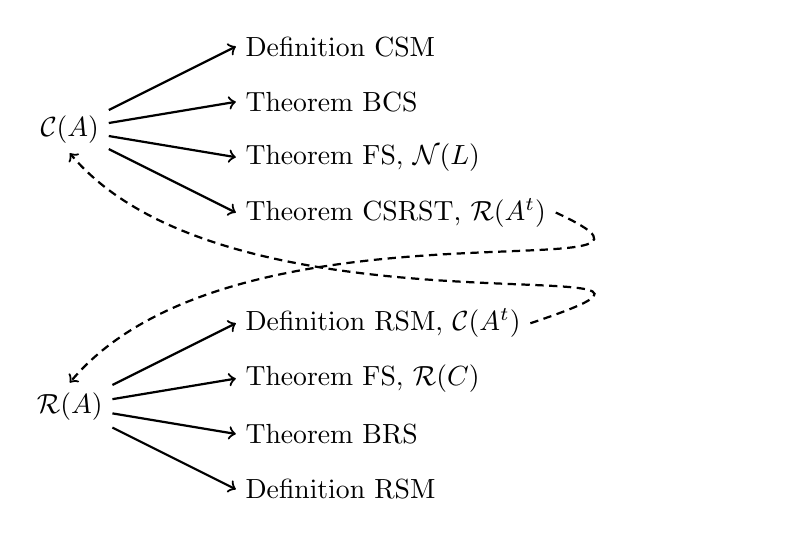
\begin{tikzpicture}
\node (CA)  at (0em, 13em) [shape=rectangle] {$\csp{A}$};
\node (CSM) at (6em, 16em) [shape=rectangle, anchor=west] {Definition CSM};
\node (BCS) at (6em, 14em) [shape=rectangle, anchor=west] {Theorem BCS};
\node (FSL) at (6em, 12em) [shape=rectangle, anchor=west] {Theorem FS, $\nsp{L}$};
\node (CSR) at (6em, 10em) [shape=rectangle, anchor=west] {Theorem CSRST, $\rsp{\transpose{A}}$};
\node (RA)  at (0em,  3em) [shape=rectangle] {$\rsp{A}$};
\node (RST) at (6em,  6em) [shape=rectangle, anchor=west] {Definition RSM, $\csp{\transpose{A}}$};
\node (FSC) at (6em,  4em) [shape=rectangle, anchor=west] {Theorem FS, $\rsp{C}$};
\node (BRS) at (6em,  2em) [shape=rectangle, anchor=west] {Theorem BRS};
\node (RSM) at (6em,  0em) [shape=rectangle, anchor=west] {Definition RSM};
\draw[->,thick] (CA) to  (CSM.west);
\draw[->,thick] (CA) to  (BCS.west);
\draw[->,thick] (CA) to  (FSL.west);
\draw[->,thick] (CA) to  (CSR.west);
\draw[->,thick] (RA) to  (RST.west);
\draw[->,thick] (RA) to  (FSC.west);
\draw[->,thick] (RA) to  (BRS.west);
\draw[->,thick] (RA) to  (RSM.west);
\draw[->,densely dashed,thick]
(RST.east) .. controls ([xshift=9em,yshift=3em]RST.east) and ([yshift=-1em]RST.west) ..  (CA.south);
\draw[->,densely dashed,thick]
(CSR.east) .. controls ([xshift=6.5em,yshift=-3em]CSR.east) and ([yshift=5em]RST.west) ..  (RA.north);
\end{tikzpicture}

Although we have many ways to describe a column space, there is one
tempting strategy to consider.

\begin{question}
  Is it possible to simply row-reduce a matrix directly and then use
  the columns of the row-reduced matrix as a set whose span equals the
  column space?
  \begin{multipleChoice}
    \choice{Yes.}
    \choice[correct]{No.}
  \end{multipleChoice}

  \begin{feedback}[correct]
    This tempting strategy will usually fail.  It is not possible to
    simply row-reduce a matrix directly and then use the columns of
    the row-reduced matrix as a set whose span equals the column
    space.  In other words, row operations \textit{do not} preserve
    column spaces (however row operations do preserve row spaces,
    \ref{theorem:REMRS}).
  \end{feedback}
\end{question}

\end{document}
